In this chapter, we consider a simple model of non-interacting spin-1 bosons on a lattice coupled with a lattice of localized spin-1 bosonic 'impurities'. This can be seen as analogue of the fermionic lattice kondo model. Our goal is to explore the nature boson-mediated interactions. 
\begin{equation}
    H = -t\sum_{\langle i, j\rangle, \sigma} a_{i\sigma}^{\dagger}a_{j\sigma} - J_h \sum_i S_i \cdot s_i
\end{equation}
This model can be thought of arising from a more general one involving coupling between the lattice and impurity bosons, in the low-energy limit of single particle occupation in the impurity sites. As a result, the localized spins can be treated as classical spins such that $|\vec{S}_i| = 1$, parametrized like so $\vec{S}_i = (\cos\phi_i\sin\theta_i, \sin\phi_i\sin\theta_i, \cos\theta_i)$. Note that the localized spins do not directly interact with each other in this system.

\section{Strong-coupling limit}
%%% FIG %%%
\begin{figure}[!htb]
    \centering
    \begin{subfigure}[b]{\textwidth}  %keep total sum <1 to show in same line
        \centering
        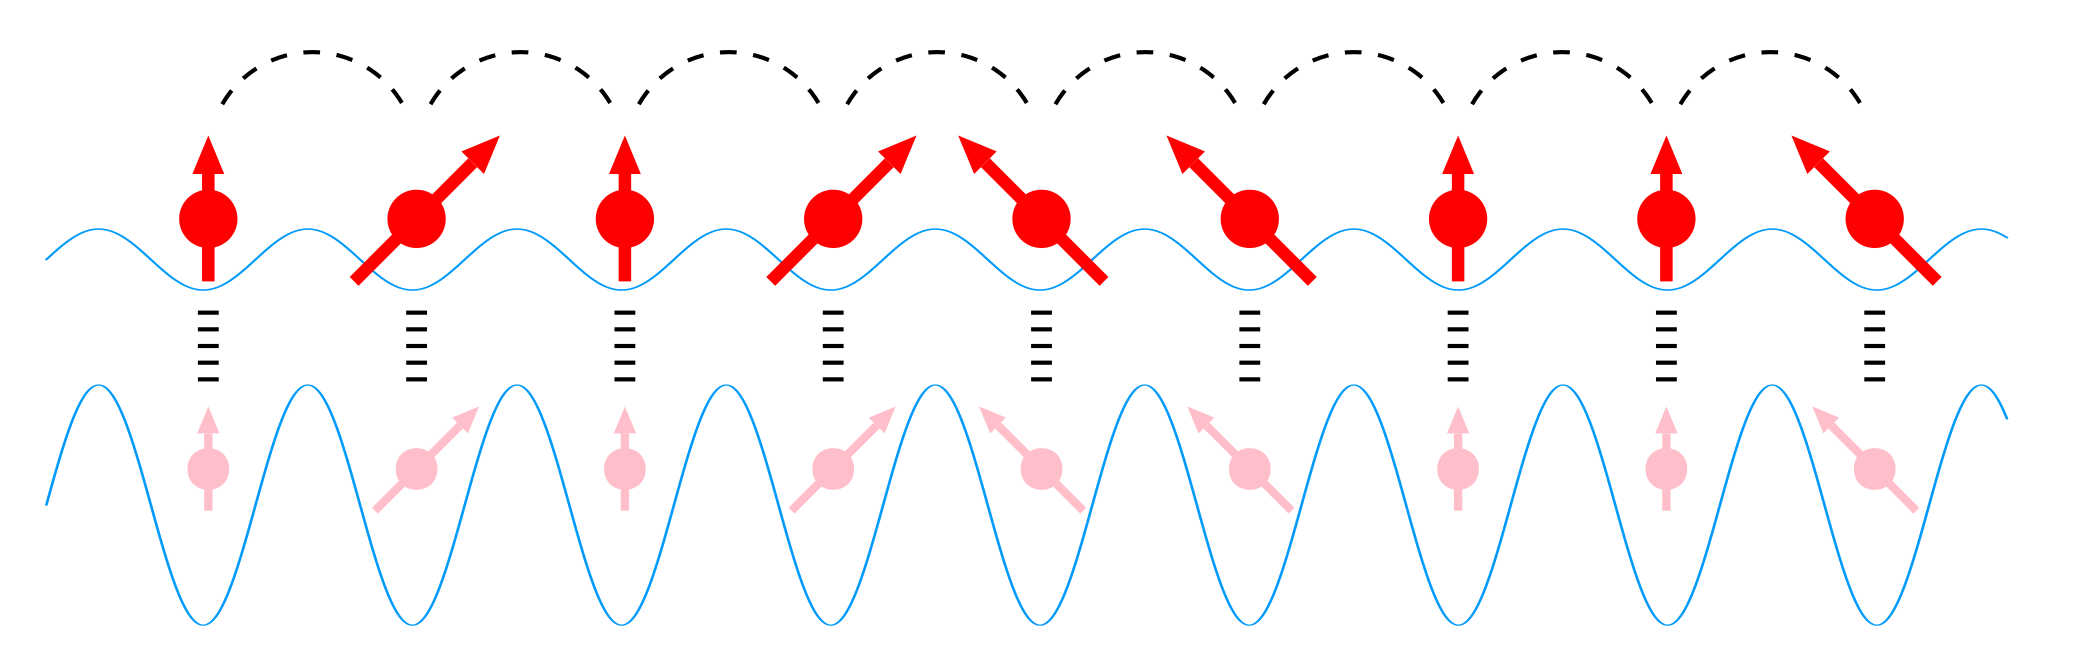
\includegraphics[width=\textwidth]{ch7/mediation.png}
    \end{subfigure}
    \caption{Conduction bosons (red) and impurity bosons (pink) confined in a lattice}
    \label{}
\end{figure}
%%% FIG %%%
\FloatBarrier \!\!\!\!\!\!\!\!\!\!\!

Let us consider the limit $J_h \gg t$ wherein the bosons have a strong tendency to align with the classical spins. This motivates us to change our basis by applying a site-dependant $SU(2)$ rotation (see Appendix \ref{app:rotation}).

\begin{equation}
    \begin{bmatrix}
        a_{i, 1} \\
        a_{i, 0} \\ 
        a_{i, \overline{1}}
    \end{bmatrix} = 
    \begin{bmatrix}
        \cos^2\frac{\theta_i}{2} & -\frac{1}{\sqrt{2}} \sin\theta_i e^{-i\phi_i} & \sin^2\frac{\theta_i}{2}e^{-2i\phi_i} \\ 
        \frac{1}{\sqrt{2}} \sin\theta_i e^{i\phi_i} & \cos\theta_i & -\frac{1}{\sqrt{2}} \sin\theta_i e^{-i\phi_i} \\
        \sin^2\frac{\theta_i}{2}e^{2i\phi_i} & \frac{1}{\sqrt{2}} \sin\theta_i e^{i\phi_i} & \cos^2\frac{\theta_i}{2}
    \end{bmatrix}
    \begin{bmatrix}
        d_{i, 1} \\
        d_{i, 0} \\ 
        d_{i, \overline{1}}  
    \end{bmatrix}
\end{equation}
The new operator, $d_{i, \sigma}$, annihilates a boson at site $i$ with the spin $\sigma \in [1, 0, \overline{1}]$ such that the quantization axis is now parallel to the localized spin. The transformed Hamiltonian can then be written as follows.
\begin{equation}
    H = \underbrace{\sum_{\langle i, j\rangle \sigma \sigma'}g_{ij}^{\sigma \sigma'} d_{i\sigma}^{\dagger} d_{j\sigma'}}_{V} - \underbrace{J_H\sum_i (n_{i,1} - n_{i, \overline{1}})}_{H_0}
\end{equation}
where $n_{i, \sigma}$ are the defined by $d_{i, \sigma}^{\dagger} d_{i, \sigma}$. Note that this transformation effectively diagonalizes the spin coupling term, which allows us to treat the hopping term in a perturbative manner. Although the elements of the new hopping matrix are not particularly insightful, they are listed below (as a multiple of $t_{i, j}$) for completeness.

\begin{align*}
    g_{i, j}^{1, 1} &= \cos^2 \frac{\theta_i}{2} \cos ^2  \frac{\theta_j}{2}  + \frac{1}{2}e^{-i(\phi_i - \phi_j)}\sin\theta_i\sin\theta_j + e^{-2i(\phi_i - \phi_j)}\sin^2 \frac{\theta_i}{2} \sin^2 \frac{\theta_j}{2}\\
%
    g_{i, j}^{1, 0} &= \frac{1}{\sqrt{2}}e^{-i\phi_i}\sin\theta_i\cos\theta_j - \frac{1}{\sqrt{2}}e^{-i\phi_j}\cos^2\frac{\theta_i}{2}  \sin\theta_j + \frac{1}{\sqrt{2}}e^{-i(2\phi_i - \phi_j)} \sin ^2  \frac{\theta_i}{2} \sin\theta_j\\
%    
    g_{i, j}^{1, \overline{1}} &=  e^{-2i\phi_i} \cos^2\frac{\theta_j}{2}\sin^2\frac{\theta_i}{2} + e^{-2i\phi_j}\cos^2\frac{\theta_i}{2}\sin^2\frac{\theta_j}{2} - \frac{1}{2}e^{-i(\phi_i + \phi_j)}\sin\theta_i\sin\theta_j\\
%   
    g_{i, j}^{0, 0} &=  \cos\theta_i\cos\theta_j + \frac{1}{2}e^{i(\phi_i - \phi_j)}\sin\theta_i\sin\theta_j + \frac{1}{2}e^{-i(\phi_i - \phi_j)}\sin\theta_i\sin\theta_j \\
%    
    g_{i, j}^{0, \overline{1}} &=  \frac{1}{\sqrt{2}}e^{-i\phi_i}\cos^2\frac{\theta_j}{2}\sin\theta_i - \frac{1}{\sqrt{2}}e^{-i\phi_j}\cos\theta_i\sin\theta_j - \frac{1}{\sqrt{2}}e^{-i(-\phi_i + 2\phi_j)}\sin\theta_i\sin^2\frac{\theta_j}{2}\\
%    
    g_{i, j}^{\overline{1}, \overline{1}} &= \cos^2\frac{\theta_i}{2}\cos^2\frac{\theta_j}{2} + \frac{1}{2}e^{i(\phi_i - \phi_j)}\sin\theta_i\sin\theta_j + e^{2i(\phi_i - \phi_j)}\sin^2\frac{\theta_i}{2}\sin^2\frac{\theta_j}{2}
\end{align*}

The remaining elements can be computed by using the property $g_{i, j}^{\sigma, \sigma'} = (g_{j, i}^{\sigma', \sigma})^*$. These coefficients can be understood as the spin-spin coupling resulting in an effective (reduced) hopping term. Let us now consider a simple case of unit occupation on the lattice, and further, we restrict the analysis to a two-site problem. The ground state for the unperturbed system is then triply degenerate.
$$\ket{0, 2} = d_{2, 1}^{\dagger}d_{2, 1}^{\dagger}\ket{0} \hspace{1cm} \ket{2, 0} = d_{1, 1}^{\dagger}d_{1, 1}^{\dagger}\ket{0}\hspace{1cm}\ket{1, 1} = d_{2, 1}^{\dagger}d_{1, 1}^{\dagger}\ket{0}$$

with energy $E_0^{(0)} = -2J_h$. Since the ground state is degenerate, we must diagonalize $V$ within this subspace to calculate the first order correction to the ground state energy. The details to compute the vacuum expectation values can be found in Appendix \ref{app:wick}. We can then write the matrix elements of $V$ in this subspace as follows.
\begin{equation}
    \bra{l, l'}V\ket{m,m'} = g_{m'l'}^{1,1} \delta_{lm} + g_{m'l}^{1,1}\delta_{l'm} + g_{ml'}^{1,1}\delta_{lm'} + g_{ml}^{1,1} \delta_{l'm'}
\end{equation}

\begin{equation}
    V = 2\Re
\begingroup
\renewcommand*{\arraystretch}{1.5}
\begin{pmatrix}
    g_{1,1}^{1,1} + g_{2, 2}^{1, 1} & 2 g_{1, 2}^{1, 1} & 2g_{2, 1}^{1, 1}\\
    2 g_{1, 2}^{1, 1} & 4t_{1, 1}^{1, 1} & 0 \\
    2g_{2, 1}^{1, 1} & 0 & 4g_{2,2}^{1, 1}
\end{pmatrix}
\endgroup
= 4
\begingroup
\renewcommand*{\arraystretch}{1.5}
\begin{pmatrix}
    0 & \Re(g_{1, 2}^{1, 1}) & \Re((g_{1, 2}^{1, 1})^*)\\
    \Re(g_{1, 2}^{1, 1}) & 0 & 0 \\
    \Re((g_{1, 2}^{1, 1})^*) & 0 & 0
\end{pmatrix}
\endgroup
\end{equation}
The smallest eigenvalue is the first order correction, $E_0^{(1)}=-4\sqrt{2}\Re(g_{1, 2}^{1, 1})$, giving us the following expression.
\begin{align}
E_0^{(1)}(\theta_i, \phi_i, \theta_j, \phi_i) = -4\sqrt{2}t_{i, j}&\left [ \cos^2\frac{\theta_i}{2}\cos^2\frac{\theta_j}{2} + \frac{1}{2}\cos(\phi_i - \phi_j)\sin\theta_i \sin\theta_j \right . \nonumber\\
&\left .+ \cos(2(\phi_i - \phi_j))\sin^2\frac{\theta_i}{2}\sin^2\frac{\theta_j}{2}\right ]    
\end{align}

Note that we have 'integrated out' the bosonic part of the system and ended up with an expression for the corrected energy purely in terms of the components of the localized spins. Thus, we have $H_{\text{eff}}({\theta_i, \phi_i, \theta_j, \phi_j}) = E_0^{(1)}(\theta_i, \phi_i, \theta_j, \phi_j) + E_0^{(0)}$ as an effective Hamiltonian governing the physics of the localized spins. We can also clearly see that the two spin variables are coupled in a non-trivial manner, thereby acting as an effective interaction that is mediated by the lattice bosons! 
\vspace{0.5cm}\\
Such a claim can be seen more clearly if we recast the effective Hamiltonian by inverting the spherical coordinates to the (cartesian) components of the localized spins.
\begin{equation}
    S_i^x = \cos\phi_i\sin\theta_i \hspace{1cm} S_i^y = \sin\phi_i\sin\theta_i \hspace{1cm} S_i^z = \cos\theta_i
\end{equation}
Unfortunately, it turns out that the first order correction cannot be neatly inverted in this manner. However, such a structure does emerge in the second order correction which roughly has the following form:
$$\sum_{\dots}(...) \cdot \frac{|g_{i, j}^{\sigma,\sigma'}|^2}{E - E_0}$$
Below is the matrix of these mod squared values that have been inverted in terms of the cartesian spin components.
\begin{equation}
    |g_{ij}^{\sigma\sigma'}|^2 = 
\begingroup
\renewcommand*{\arraystretch}{1.5}
\frac{t_{i, j}^2}{4}\begin{bmatrix}
    (1 + \vec{S}_i \cdot \vec{S}_j)^2 & 2(1 - (\vec{S}_i \cdot \vec{S}_j)^2) & (1 - \vec{S}_i \cdot \vec{S}_j)^2 \\ 
    2(1 - (\vec{S}_i \cdot \vec{S}_j)^2) & 4(\vec{S}_i \cdot \vec{S}_j)^2 & 2(1 - (\vec{S}_i \cdot \vec{S}_j)^2) \\
    (1 - \vec{S}_i \cdot \vec{S}_j)^2 & 2(1 - (\vec{S}_i \cdot \vec{S}_j)^2) & (1 + \vec{S}_i \cdot \vec{S}_j)^2
\end{bmatrix}
\endgroup
\end{equation}   
We can clearly see a much nicer interpretation of the mediated interaction since these represent Heisenberg-like couplings between the localized spins. However, we do not pursue the complete calculation since the leading order correction is non-zero.

% \begin{equation}
% \wick{
% \c1 a \c2 b \c3 c \c1 a \c4 d \c1 e
% \c1 e \c1 a \c2 b \c3 c \c1 a
% }
% \end{equation}